%!TEX root = ../main.tex

%=======================================================================  numbers
\section{Numbers}
\label{sec:numbers}

	In the beginning, we must define the main players in the world of math: numbers.

	\subsection{Definitions}
	\label{numbers:definitions}
		
		Numbers are the basic objects we use to count, measure, quantify, and calculate things.
		Mathematicians like to classify the different kinds of number-like objects into categories called \emph{sets}:					\index{set}
		\begin{itemize}
			\item  The natural numbers: $\mathbb{N} = \{0,1,2,3,4,5,6,7, \ldots \, \}$
			\item  The integers: $\mathbb{Z} = \{\ldots, -3,-2,-1,0,1,2,3 , \ldots  \, \}$
			\item  The rational numbers: $\mathbb{Q} = \{\frac{5}{3}, \frac{22}{7}, 1.5, 0.125,  -7, \, \ldots \, \}$
			\item  The real numbers: $\mathbb{R} = \{-1,0,1, \sqrt{2}, e,\pi, \;  4.94\ldots, \; \ldots \, \}$
			\item  The complex numbers: $\mathbb{C} = \{ -1, 0, 1, i,  1+i, 2+3i,  \ldots \, \}$
		\end{itemize}
		%
		These categories of numbers should be somewhat familiar to you.
		Think of them as neat classification labels for everything that you would normally call a number. 
	 	Each group in the above list is a \emph{set}.
		A set is a collection of items of the same kind. 
		Each collection has a name and a precise definition for which items belong in that collection.
		Note also that each of the sets in the list contains all the sets above it,												\index{set!subset}
		as illustrated in Figure~\ref{fig:nested_sets}.
		For now, we don't need to go into the details of \hyperref[sec:set_notation]{sets and set notation},
		but we do need to be aware of the different sets of numbers.

		\begin{figure}[H]
			\centering
			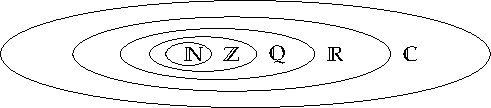
\includegraphics[width=0.87\textwidth]{figures/math/nested_sets.pdf}
			\caption{	An illustration of the nested containment structure of the different number sets.
					The set of natural numbers is contained in the set of integers,
					which in turn is contained in the set of rational numbers.
					The set of rational numbers is contained in the set of real numbers,
					which is contained in the set of complex numbers.}
			\label{fig:nested_sets}
		\end{figure}

		\noindent
		Why do we need so many different sets of numbers?
		Each set of numbers is associated with more and more advanced mathematical problems.

		The simplest numbers are the natural numbers $\mathbb{N}$,
		which are sufficient for all your math needs if all you're going to do is \emph{count} things.
		How many goats? Five goats here and six goats there so the total is 11 goats. 
		The sum of any two natural numbers is also a natural number.

		As soon as you start using \emph{subtraction} (the inverse operation of addition),
		you start running into negative numbers,
		which are numbers outside the set of natural numbers.
		If the only mathematical operations you will ever use are \emph{addition} and \emph{subtraction},
		then the set of integers $\mathbb{Z} = \{ \ldots, -2, -1, 0, 1, 2, \ldots \}$ will be sufficient.
		Think about it.
		Any integer plus or minus any other integer is still an integer.

		You can do a lot of interesting math with integers.
		There is an entire field in math called \emph{number theory} that deals with integers.
		However, to restrict yourself solely to integers is somewhat limiting---a rotisserie
		menu that offers $\frac{1}{2}$ of a chicken would be totally confusing.

		If you want to use division in your mathematical calculations,														\index{rational}
		you'll need the rationals~$\mathbb{Q}$.
		The set of rational numbers corresponds to all numbers that can be expressed as \emph{fractions} of the form $\frac{m}{n}$		\index{fraction}
		where $m$ and $n$ are integers, and $n \neq 0$.
		You can add, subtract, multiply, and divide rational numbers, and the result will always be a rational number.
		However, even the rationals are not enough for all of math!

		In geometry, we can obtain \emph{irrational} quantities like $\sqrt{2}$ (the diagonal of a square with side 1)
		and $\pi$ (the ratio between a circle's circumference and its diameter).
		There are no integers $x$ and $y$ such that $\sqrt{2}=\frac{x}{y}$,
		therefore we say that $\sqrt{2}$ is \emph{irrational} (not in the set $\mathbb{Q}$).
		An irrational number has an infinitely long decimal expansion that doesn't repeat.
		For example, $\pi = 3.141592653589793\ldots$ where the dots indicate
		that the decimal expansion of $\pi$ continues all the way to infinity.

		Combining the irrational numbers with the rationals gives us all the useful numbers,
		which we call the set of real numbers $\mathbb{R}$.
		The set $\mathbb{R}$ contains the integers,
		the rational numbers $\mathbb{Q}$,
		as well as irrational numbers like $\sqrt{2}=1.4142135\ldots$.
		By using the reals you can compute pretty much anything you want.
		From here on in the text, when I say \emph{number},
		I mean an element of the set of real numbers $\mathbb{R}$.

		The only thing you can't do with the reals is to take the square root of a negative number---you 							\index{complex number}
		need the complex numbers $\mathbb{C}$ for that.
		We defer the discussion on $\mathbb{C}$ until the end of Chapter~\ref{chapter:vectors}.


	\subsection{Exercises}
	\label{numbers:exercises}
	
		%!TEX root = ../main.tex

\begin{exercises}{ch1}	


	\begin{exercise}
		Solve for the unknown $x$ in the following equations:

		\twocol
		\textbf{a)}~$3x+2-5=4+2$

		\textbf{b)}~$\frac{1}{2}x-3=\sqrt{3}+12-\sqrt{3}$
		\endtwocol

		\twocol
		\textbf{c)}~$\frac{7x-4}{2} +1 = 8-2$
		
		\textbf{d)}~$5x-2+3=3x-5$
		\endtwocol
				
		\begin{eanswer}\textbf{a)}~$x=3$; \textbf{b)}~$x=30$; \textbf{c)}~$x=2$; \textbf{d)}~$x=-3$.\end{eanswer}
					\end{exercise}


	\begin{exercise}
		Indicate all the number sets the following numbers belong to.
				
		\fivecol
		\textbf{a)}~$-2$ 

		\textbf{b)}~$\sqrt{-3}$
		
		\textbf{c)}~$8 \div 4$
		
		\textbf{d)}~$\frac{5}{3}$
		
		\textbf{e)}~$\frac{\pi}{2}$
		
		\endfivecol
		
		\begin{eanswer}\textbf{a)}~$\mathbb{Z}, \mathbb{Q}, \mathbb{R},\mathbb{C}$;
					\textbf{b)}~$\mathbb{C}$;
					\textbf{c)}~$\mathbb{N},\mathbb{Z}, \mathbb{Q}, \mathbb{R},\mathbb{C}$;
					\textbf{d)}~$\mathbb{Q}, \mathbb{R},\mathbb{C}$;
					\textbf{e)}~$\mathbb{R},\mathbb{C}$.\end{eanswer}
					\end{exercise}

	

	\begin{exercise}
		Calculate the values of the following expressions:
		
		\threecol
		\textbf{a)}~$2^33-3$ 

		\textbf{b)}~$2^3(3-3)$
		
		\textbf{c)}~$\frac{4-2}{3^3}(6\cdot 7- 41)$
		\endthreecol
		
		\begin{eanswer}\textbf{a)}~$21$; \textbf{b)}~$0$; \textbf{c)}~$\frac{2}{27}$.\end{eanswer}
					\end{exercise}	



\end{exercises}

	

